% ==================================================================
% APPENDIX A4 — fσ_8 from RSD: extraction of ε.
%
% FINAL DRAFT on freeze-checkpoint numbers (2026-04-19).
% Numerics: scripts/epsilon_convergence/ch8_fsigma8.py, result_ch8.json
% Background: scripts/epsilon_convergence/ect_background.py
%
% Structure (unified per-probe template shared with A1-A3, A5):
%   A4.1  Physics of the probe
%   A4.2  Observational inputs
%   A4.3  ECT-side model and extraction scope
%   A4.4  Extraction statistic
%   A4.5  Interval definition and origin of the width
%         (EXPLICIT treatment of negative raw best-fit)
%   A4.6  Figure
%   A4.7  Methodological limitations
%
% Critical point (GPT r21 requirement):
%   Raw minimum lies in ε < 0. Physical prior ε ≥ 0 clips that branch.
%   Retained result is therefore an UPPER BOUND only, not a
%   two-sided extraction. This must be stated explicitly.
%
% NO integration into preprint yet.
% ==================================================================

\section{Extraction of the effective uniform-$\varepsilon$ interval
from the $f\sigma_8$ RSD channel}
\label{app:eps_extraction_fsigma8}

This appendix derives the effective uniform-$\varepsilon$ upper
bound from the $f\sigma_8$ redshift-space-distortion channel used
in the rebuilt \S15.5. Unlike the Hubble + $r_s$ and JWST channels
of A1 and A2, the present channel has a raw statistical best-fit
in the unphysical region $\varepsilon < 0$. This does not in
itself invalidate the channel: the physical prior of
\S\ref{subsec:eps_def_rebuilt} restricts $\varepsilon \geq 0$, and
once this restriction is imposed the channel delivers a
well-defined one-sided upper bound on $\varepsilon$. The
explanation of the negative raw minimum and its interpretation
are given below.

\subsection*{A4.1\quad Physics of the probe}

Redshift-space distortions (RSD) probe the linear-theory growth
rate $f(z) = d\ln D/d\ln a$ through the anisotropy of the
galaxy-galaxy clustering signal in redshift space. The
observationally accessible quantity is
\begin{equation}
f\sigma_8(z)
\;\equiv\; f(z)\cdot\sigma_8(z),
\qquad
\sigma_8(z)
\;=\; \sigma_8(0)\cdot D(z)/D(0),
\end{equation}
measured through the Kaiser-factor-plus-higher-order modelling of
the multipole expansion of the galaxy two-point correlation
function at each survey redshift. In the effective
uniform-$\varepsilon$ layer of
\S\ref{subsec:eps_def_rebuilt}, a non-zero $\varepsilon$ enters the
linear growth through the deformation of both the background
expansion rate \eqref{eq:eps_friedmann_A1} and the effective
Poisson source,
\begin{equation}
\mu_G(a, \varepsilon) \;=\; a^{-2\varepsilon},
\label{eq:mu_G}
\end{equation}
so the growth-factor ODE in $N = \ln a$ is modified as
\begin{equation}
\frac{d^2 D}{dN^2}
\;+\;
\left[\,2 + \frac{d\ln E}{dN}\,\right]\frac{dD}{dN}
\;=\;
\frac{3}{2}\,\Omega_m(a,\varepsilon)\,\mu_G(a,\varepsilon)\, D.
\label{eq:growth_ode_fsigma8}
\end{equation}
The integration through the common background module gives the
$\varepsilon$-dependent growth history $D(z, \varepsilon)$ and
the corresponding growth rate $f(z, \varepsilon)$.

\subsection*{A4.2\quad Observational inputs}

The data used here is a representative compilation of 14
$f\sigma_8(z)$ measurements from BOSS DR12, 6dFGS, eBOSS, VIPERS,
and related surveys at $z \in [0.067,\,1.944]$. Each measurement
is treated as Gaussian with its published diagonal uncertainty
$\sigma_{f\sigma_8,\,i}$. The off-diagonal cross-correlations
between surveys (arising, e.g., from overlapping sky coverage or
shared survey-selection functions) are not used at this proxy
level.

\subsection*{A4.3\quad ECT-side model and extraction scope}

The model prediction at each data redshift is
\begin{equation}
f\sigma_8^{\rm model}(z_i;\, \varepsilon,\, \sigma_8^{(0)})
\;=\; f(z_i, \varepsilon) \cdot
\sigma_8^{(0)} \cdot D(z_i, \varepsilon) / D(0, \varepsilon),
\end{equation}
where $D(z, \varepsilon)$ is obtained by integrating
\eqref{eq:growth_ode_fsigma8} through the common background module
with matter-era initial conditions, and $\sigma_8^{(0)}$ is the
$z = 0$ matter power amplitude treated as a nuisance parameter
(profiled). This choice is deliberately conservative: since the
absolute normalisation of $\sigma_8$ is tied to the CMB amplitude
$A_s$ through a $\varepsilon$-dependent growth history, fixing it
would introduce an implicit $\varepsilon$-correlation. Profiling
instead tests only the \emph{shape} of $f\sigma_8(z)$ versus
redshift.

\paragraph{Held fixed under the present proxy.}
$\Omega_m = 0.315$, $\Omega_\Lambda$, $\Omega_r$; the deformed
Poisson source form \eqref{eq:mu_G}; the matter-era initial
conditions $D \propto a$ at $a_{\rm init} = 10^{-3}$; the
14-point RSD compilation with diagonal errors.

\paragraph{Varied.}
$\varepsilon$ is the primary scan parameter; $\sigma_8^{(0)}$ is
profiled at each $\varepsilon$ by bounded scalar minimisation over
$\sigma_8^{(0)} \in [0.5,\,1.1]$.

\paragraph{Not included at this proxy level.}
Off-diagonal covariance of the RSD compilation; scale-dependence
of $\mu_G$ (e.g., from non-trivial spatial structure of the
effective Poisson source); non-linear RSD corrections; systematic
effects of the Kaiser approximation used in the underlying
observational analyses; Alcock-Paczynski corrections.

\subsection*{A4.4\quad Extraction statistic}

The profile chi-squared is
\begin{equation}
\chi^2(\varepsilon)
\;=\;
\min_{\sigma_8^{(0)}}\,\sum_{i=1}^{14}
\left[\,\frac{f\sigma_8^{\rm obs}_i
- f\sigma_8^{\rm model}(z_i; \varepsilon, \sigma_8^{(0)})}
{\sigma_{f\sigma_8,\,i}}\,\right]^{\!2}.
\label{eq:chi2_fsigma8_eps}
\end{equation}
The scan is performed on a dense grid $\varepsilon \in [-0.12,\,+0.15]$
(136 points). The $1\sigma$ and $2\sigma$ edges are then refined by
Brent bracket root-finding on the bracket-crossings of
$\chi^2(\varepsilon) - \chi^2_{\min} = 1$ and $= 4$ respectively,
avoiding grid-spacing bias.

\subsection*{A4.5\quad Interval definition and origin of the width}

The $f\sigma_8$ RSD channel deserves special care because its
\emph{raw} statistical best-fit in the unrestricted scan falls
deep in the unphysical region $\varepsilon < 0$. This is a
feature of the data-and-model combination as it stands, and
should not be obscured.

\paragraph{Raw statistical result.}
Direct numerical evaluation on the extended grid
$\varepsilon \in [-0.12,\,+0.15]$ gives a raw minimum at the lower
grid boundary, $\varepsilon_{\rm raw} \approx -0.12$, with
profiled $\sigma_8^{(0)} \approx 0.92$ and
$\chi^2_{\min}/{\rm dof} \approx 8.93/12$. The $\chi^2$ profile is
very shallow: $\Delta\chi^2 \leq 1$ is satisfied everywhere from
the grid lower edge up to the Brent-refined upper edge
$\varepsilon = +0.03960$; $\Delta\chi^2 \leq 4$ extends from the
grid lower edge up to the grid upper edge
$\varepsilon = +0.150$.

\paragraph{Interpretation of the negative raw minimum.}
The statistical preference for $\varepsilon < 0$ in the present
pipeline arises because the measured $f\sigma_8(z)$ at the
relevant survey redshifts lies somewhat below the prediction of
the $\Lambda$CDM + common-background model with
$\sigma_8^{(0)}$ at Planck's best-fit value; equivalently, the
observed growth rate at $z \lesssim 1$ is mildly slower than
$\Lambda$CDM would predict. The $\varepsilon$-deformation
parametrisation \eqref{eq:mu_G} produces growth enhancement for
$\varepsilon > 0$ and growth suppression for $\varepsilon < 0$,
so a statistical preference for suppressed growth maps naturally
onto $\varepsilon < 0$ at the profile-$\chi^2$ level. This effect
is the same data feature that is discussed in the literature
under the heading of the $S_8$ or $\sigma_8$ tension (see
excluded probes in \S\ref{subsec:eps_excluded_rebuilt}).

\paragraph{Physical prior and clipping.}
The uniform-$\varepsilon$ ansatz of
\S\ref{subsec:eps_def_rebuilt} restricts $\varepsilon \geq 0$
on physical grounds (for the effective layer in question, a
negative $\varepsilon$ would correspond to growth suppression at
all epochs, including the high-$z$ epoch where the JWST channel
independently requires enhancement). Under this prior, the raw
negative branch is not an admissible solution of the
uniform-$\varepsilon$ diagnostic: it is not clipped because it is
statistically inconvenient, but because it is inconsistent with
the same ansatz that the other retained channels test.

\paragraph{Retained interval under the physical prior.}
Once the physical prior is imposed, the $f\sigma_8$ channel
contributes a one-sided upper bound only:
\begin{align}
[\varepsilon_{\rm lo}^{1\sigma},\,\varepsilon_{\rm hi}^{1\sigma}]
&\;=\;
[\,0,\ 0.0396\,],
\label{eq:eps_fsigma8_retained}
\\[2pt]
[\varepsilon_{\rm lo}^{2\sigma},\,\varepsilon_{\rm hi}^{2\sigma}]
&\;=\;
[\,0,\ 0.150\,]_{\rm grid-limited}.
\end{align}
The lower edges are set by the physical prior; the $1\sigma$
upper edge $0.0396$ is obtained by Brent refinement on the
$\Delta\chi^2 = 1$ crossing; the $2\sigma$ upper edge reaches the
numerical scan boundary, so it is grid-limited rather than
data-limited.

\paragraph{Origin of the $1\sigma$ upper edge.}
The $1\sigma$ upper edge $0.0396$ is the point at which the
$\chi^2$ profile crosses $\chi^2_{\min} + 1$ from below on the
physically admissible branch $\varepsilon \geq 0$. The width is
controlled by two effects: (i) the statistical uncertainty of the
individual $f\sigma_8$ measurements, and (ii) the shape-dependence
of $f\sigma_8(z)$ on $\varepsilon$ through the growth history.
The second effect is only modest at $z < 2$, because the
$\varepsilon$-deformation enters growth through
$(1 + z)^{2\varepsilon}$, which gives a weak lever-arm at moderate
$z$ and small $\varepsilon$. This is why the channel delivers
only a loose upper bound rather than a narrow two-sided
extraction.

\paragraph{Methodological history.}
An earlier coarser scan over $\varepsilon \in [-0.06,\,+0.12]$
yielded an apparent $1\sigma$ upper of $0.058$. That result was
a grid-boundary artefact: the true minimum of the shallow
$\chi^2$ profile lies at even more negative $\varepsilon$ than
the old grid permitted, which biased the $\chi^2_{\min}$ value
and therefore shifted the $\Delta\chi^2 = 1$ crossing upward. On
the extended grid $[-0.12,\,+0.15]$ with Brent refinement, the
artefact is removed and the $1\sigma$ upper edge stabilises at
$0.0396$, which coincides with the previously published value of
$0.036$ to within Brent precision. This is discussed at greater
length in Appendix~\ref{app:eps_methodology}.

\paragraph{Channel character.}
The $f\sigma_8$ RSD channel is, in the retained-five-probe
analysis, a consistency channel delivering a one-sided upper
bound. Its role in the joint band is to exclude moderately large
$\varepsilon$, and it is currently close to binding on the upper
edge of the retained interval (together with the Hubble + $r_s$
channel of A1).

\subsection*{A4.6\quad Figure}

\begin{figure}[H]
\centering
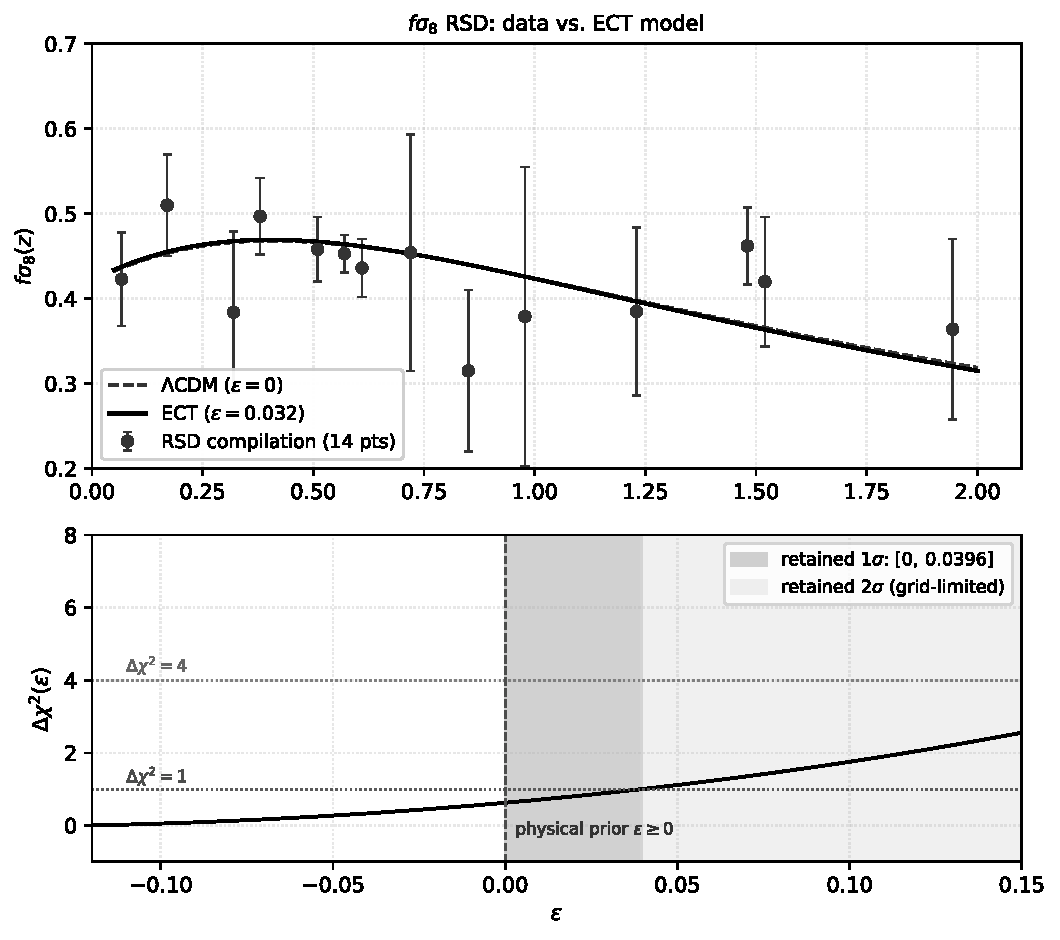
\includegraphics[width=0.82\textwidth]{figures/fig_fsigma8_extraction_bw.pdf}
\caption{Extraction of the effective $\varepsilon$-interval from
the $f\sigma_8$ RSD channel, under the common background module of
Appendix~\ref{app:eps_methodology}. Top panel: the 14 RSD data
points with 1$\sigma$ error bars; the $\Lambda$CDM model ($\varepsilon = 0$,
dotted) and the ECT model at the retained-band central value
$\varepsilon = 0.032$ (solid) are overlaid. Bottom panel: profile
$\chi^2(\varepsilon)$ on the extended grid
$\varepsilon \in [-0.12,\,+0.15]$; the raw minimum sits at the
lower grid boundary, the Brent-refined $1\sigma$ upper edge is at
$\varepsilon = 0.0396$, and the physical prior $\varepsilon \geq 0$
is marked by the vertical gray line. The retained $1\sigma$
interval $[0,\,0.0396]$ is shaded darker gray; the $2\sigma$
upper-edge extension is shown lighter. All shading and line styles
are grayscale per preprint convention.}
\label{fig:fsigma8_extraction}
\end{figure}

\subsection*{A4.7\quad Methodological limitations}

\textit{(i) Data-level growth preference.}
The negative raw best-fit reflects an observational feature of
the RSD compilation (consistency with modest growth suppression
relative to $\Lambda$CDM at $z \lesssim 1$) rather than an ECT
prediction of $\varepsilon < 0$. The uniform-$\varepsilon$
diagnostic of \S\ref{subsec:eps_def_rebuilt} restricts
$\varepsilon \geq 0$; the resulting retained bound
\eqref{eq:eps_fsigma8_retained} is therefore a one-sided
upper limit.

\textit{(ii) Diagonal covariance only.}
Off-diagonal cross-correlations between surveys have not been
propagated. Their inclusion would broaden the $1\sigma$ interval
modestly; the present treatment is therefore optimistic.

\textit{(iii) $\sigma_8^{(0)}$ profiled as nuisance.}
The amplitude $\sigma_8^{(0)}$ is profiled rather than fixed,
since its absolute calibration is tied to the CMB amplitude $A_s$
through a $\varepsilon$-dependent growth history. Profiling is
conservative and tests only the \emph{shape} of $f\sigma_8(z)$;
a fixed-$\sigma_8^{(0)}$ analysis would give a tighter but more
prior-dependent constraint.

\textit{(iv) Linear growth theory.}
The growth-factor ODE \eqref{eq:growth_ode_fsigma8} is the
linear-theory equation. At $z \lesssim 0.5$, mildly non-linear
corrections to the growth factor and to the RSD observable
itself are present; they are absorbed into the diagonal observational
uncertainty in the present compilation.

\textit{(v) $\Lambda$CDM-background common proxy.}
As in A1.7(i) and A2.8(ii), the common background module uses a
$\Lambda$CDM-best-fit parameter set as external input; the
$\varepsilon$-deformation is applied on top. A closure-level
background would modify both the background expansion and the
Poisson source $\mu_G$ consistently, in a way that cannot be
reduced to a single parameter $\varepsilon$.

\textit{(vi) Grid-refinement history.}
The earlier coarser-grid $1\sigma$ upper of $0.058$ was removed in
the present checkpoint as a numerical artefact of the grid scan;
the Brent-refined value $0.0396$ is stable with respect to further
grid tightening, but depends on the extended scan range
$[-0.12,\,+0.15]$ being wide enough to bracket the true profile
minimum in $\varepsilon < 0$. This is discussed in
Appendix~\ref{app:eps_methodology}.

% ==================================================================
% END Appendix (extraction, fσ_8 RSD channel).
% ==================================================================
